\documentclass[11pt,a4paper]{vutinfth}
\usepackage[utf8]{inputenc}
\usepackage{graphicx}
\usepackage{textcomp}
\usepackage{caption}
\usepackage{mathtools}
\usepackage{amssymb}
\usepackage[boxed,linesnumbered]{algorithm2e}
\usepackage{color}
%\usepackage[]{luatodonotes}
%\usepackage{wrapfig}



%TODO: CHANGE!
\setauthor{}{Jakob Klinger}{}{male}
\setadvisor{Ass.Prof. Dipl.-Inform. Dr.rer.nat}{Martin Nöllenburg}{}{male}%{Pretitle}{Forename Surname}{Posttitle}{male}
\setfirstassistant{Univ.Ass.}{Fabian Klute}{ M.Sc., B.Sc.}{male}
%Ass.Prof. Dipl.-Inform. Dr.rer.nat. Martin Nöllenburg
% University Assistant, M.Sc., B.Sc. Fabian Klute

\setaddress{Scherzergasse 10/8, 1020 Wien}
\setregnumber{1125755}
\setdate{25}{09}{2017}%TODO: Update

\settitle{Boundary Labeling for annotated documents}{Boundary Labeling in annotierten Dokumenten}
\setsubtitle{}{}%{TestSubtitleENG}{TestSubtitelGER}

\setthesis{bachelor}
\setcurriculum{Bachelor's programme Software \& Information Engineering}{Bachelorstudium Software \& Information Engineering} %TODO!



\newcommand{\change}[1]{\textcolor{red}{#1}}

\begin{document}

\frontmatter
%\addtitlepage{naustrian}
\addtitlepage{english}
\addstatementpage

%\begin{danksagung*}
%\todo{Ihr Text hier.}
%\end{danksagung*}

%\begin{acknowledgements*}
%\todo{Enter your text here.}
%\end{acknowledgements*}

%\begin{kurzfassung}
%\todo{Ihr Text hier.}
%\end{kurzfassung}

%\begin{abstract}
%\todo{Enter your text here.}
%\end{abstract}

\selectlanguage{english}

\tableofcontents

\mainmatter


%TODO: Abstract: \begin{abstract}...\end{abstract}

\chapter{Introduction}
Whenever additional information neets to be inserted into an existing document without altering the original text, we can make use of annotations. They usually take the form of footnotes, which require only a minimal reference in the main text, and are used for a variety of reasons - for example, to provide additional information that would hinder the text's flow if inserted directly, or as a result of a commenting tool that is used for communication between an author and their editor.
If a more obvious connection between the text and the referenced content is required, for example when lengthy comments are added, or if a change-tracking tool is used, the reference is often placed to the side of the document and visibly connected to the part of the text it is referring to. This style of annotation is easily implemented on virtual documents, since they can be hidden on demand, however if the annotations need to be included in a printed version, there are several issues that arise regarding readability of the final product and ambiguity of text-annotation assignments.

In this thesis, we will look at ways to use Boundary Labeling for this problem, which means that all annotations will be placed somewhere outside of the text they are referencing and will be visually connected to the feature they are referencing. (See also \cite{Bekos2007}) 

The guidelines on how to create suitable labelings are as follows: the connections should be as direct as possible, no important information should be obscured, and it should be easily discernable which Label belongs where. These three criteria easily come into conflict with one another, as the text usually is very dense and leaves little space for lines in between, yet one shouldn't allow them to pass through the text, as this makes the text harder to read. 

\section{Terminology and Fundamentals} %Evtl in Introduction eingliedern?
Boundary Labeling (or equivalent concepts) can be applied to a space with different geometry or more dimensions, but this thesis will only concern itself with two-dimensonal, Euclidean space.
To easily reference important concepts, some additional terminology will be introduced as well. (See Fig.~\ref{fig:term} for a visual explanation)


\begin{figure}%{r}{0.35\textwidth}
 \captionsetup{justification=centering, margin=0.75cm}
 \centering
  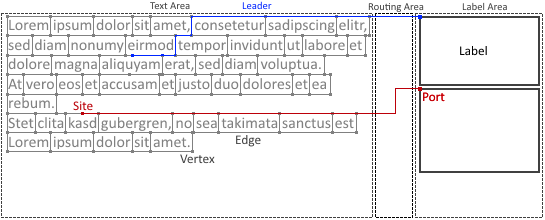
\includegraphics[scale=0.90]{GraphTerminologyExtended.png}
  \caption{Illustrated guide to the labeling terminology}
 \label{fig:term}
\end{figure}

A \emph{graph} $G=\langle V, E \rangle$ is a tuple of \emph{vertices} $V=\{v_1, v_2, ..., v_n\}$ and \emph{edges} $E=\{e_1, e_2, ..., e_m\}$. A vertex $v$ is a featureless object. %Wie  sage ich, dass die Umsetzung der Vertices sehr flexibel ist?
 Each edge $e$ is a relation between two vertices $E \subseteq V\times V$. %Edges can also be directional, or have a weight, which affects how they are treated by algorithms.
We call two vertices $u,v \in V$ \emph{adjacent}, if the edge $e=(u,v) \in E$.
 A \emph{path} $P=v_1, ..., v_h$ is an ordered sequence of vertices, where each vertex must have an edge connecting it to the subesquent one.
 \emph{Depth-first search} is a searching algorithm on a graph G that starts at a given vertex $v \in V$ and explores the graph by traversing its edges as far as possible before backtracking, and continues to do so until a pre-defined goal is met. %In our algorithm, the goal is to reach a target vertex $v_t \in V$, at which point the algorithm terminates and returns the route taken from $v_s$ to $v_t$.
% A search algorithm is \emph{monotonous} if, for each vertex $v$ and each successor $v'$ generated by the algorithm, the estimated cost of reaching the goal from $v$ is not greater than the cost of reaching $v'$ plus the estimated cost of reaching the goal from $v'$.

\emph{Polylines} are a connected series of \emph{line segments}. Line segments are straight lines that contain each point between their starting and end point. 
\emph{Labels} hold additional information and are represented as boxes containing this information. They are usually placed in the \emph{Label area} which is a rectangular area designated to hold labels. It is located next to of the bigger \emph{text area}, which contains the document's text and all \emph{sites}, the points or objects that a label's information refers to. The site and the label are connected via a \emph{leader}, a polyline that can be further classified by looking at the orientation of its segments: \emph{O-Segments} run orthogonally to the border of the label area. \emph{P-Segments} run parallel to the border of the label area, and as such must be combined with other segments for the leader to reach its destination. \emph{S-Segments} are not required to have any particular orientation, and simply connect their start and ending points in a straight line.
The leader's name is created by combining the name of the segments - for example, the blue leader from Fig~\ref{fig:term} would be classified as an OPOPO-Leader.
The location where a leader connects to the label is called the \emph{port}. It can be restricted to pre-defined positions. %TODO: Re-insert monotonicity

% \textbf{Monotonous/Monotonicity:} Describes a steady progression towards a direction or goal. Will be used in this paper to indicate that there's no loss of progress made from the site to the label, effectively restricting the direction a leader can go at each bend.
%+Node für Knoten in Polylinien?

\section{Related Work}

While there are many papers discussing Boundary Labeling in general, only very few exist that apply this concept to written text. Generally, this approach isn't used very often, and tends to use simplistic algorithms which produce mediocre results. %Beispiele von suboptimalen Lösungen einfügen? (Bilder)

The concept of boundary labeling is introduced in \cite{Bekos2007}, where several approaches with varying leader types are discussed, along with any problems that arise. 
However, the papers that do discuss boundary labeling in text offer interesting contributions.

The paper about the Luatodonotes-Package\cite{Kindermann2014} illustrates some of the different styles of drawing these connecting paths, and came to the conclusion that paths without bends are easier to follow. %Bsp-Bild einfügen!
However, most solutions proposed in that paper do not consider whether a path overlaps with text or not, which results in a decrease in readability.

The thesis by Loose\cite{Loose2015} on the other hand is based around only using the free space between lines and words, which produces longer paths, and forces curves, but doesn't obscure any part of the text.


\chapter{The Algorithm}

In our algorithm, the focus was put on keeping the text as readable as possible. This means that leaders aren't allowed to pass through words, which was implemented by enclosing each word in a bounding rectangle that leaders aren't allowed to pass through.
The leaders should also be kept as short as possible, so we restricted them to always be moving toward the label, even if the direct route is unavailable.%Wie drücke ich das als Formel aus?
We also wanted to use the space available in the labeling area as efficiently as possible, so labels are placed as far up as possible in order to maximize the space available to future labels at the cost of increased leader length.


\begin{algorithm}%{r}{0.35\textwidth}
\DontPrintSemicolon
\SetKwData{Words}{words}
\SetKwData{PrevW}{previousWord}
\SetKwData{G}{Graph}
\SetKwData{W}{w} \SetKwData{V}{v}\SetKwData{Va}{v1} \SetKwData{Vb}{v2} \SetKwData{Vc}{v3} \SetKwData{Vd}{v4}
\SetKwData{Up}{UpperVerticesList}
\SetKwData{Low}{LowerVerticesList}

\SetKwFunction{setAnn}{setAnnotation}
\SetKwFunction{NewVert}{new Vertex}
\SetKwFunction{AddVert}{addVertex}
\SetKwFunction{AddAll}{addAll}
\SetKwFunction{CEdge}{createEdgeBetween}
\SetKwFunction{PosConn}{connectBasedOnPosition}
\SetKwFunction{ClrList}{emptyList}
\SetKwFunction{getC}{getCenter}
\SetKwFunction{tLeft}{getTopLeft}
\SetKwFunction{tRight}{getTopRight}
\SetKwFunction{bLeft}{getBottomLeft}
\SetKwFunction{bRight}{getBottomRight}
\SetKwFunction{Newline}{startNewLine}

\KwData{A text with annotations,stored as a String-Array}
\KwResult{A Graph (as described above)}

 initialization\;
 
 \ForEach{\W in \Words}{
  \eIf{\W is annotation}{
   \V$\gets$\NewVert{\PrevW.\getC{}}\;
   \V.\setAnn{w}\;
   \G.\AddVert{\V}\;
   \Up.\AddVert{\V}\;
  }{
   \If{\W is too big for the line}{
    \Newline{}\;
    \PosConn{\Up}\;
    \Up$\gets$\Low\;
    \ClrList{\Low}\;
   }
   \Va $\gets$\NewVert{\W.\tLeft{}}\;
   \Vb $\gets$\NewVert{\W.\tRight{}}\;
   \Vc $\gets$\NewVert{\W.\bLeft{}}\;
   \Vd $\gets$\NewVert{\W.\bRight{}}\;
   \;
   \G.\AddAll{\Va,\Vb,\Vc,\Vd}\;
   \Up.\AddAll{\Va,\Vb}\;
   \Low.\AddAll{\Vc,\Vd}\;
   \G.\CEdge{\Va,\Vc}\;
   \G.\CEdge{\Vb,\Vd}\;
  }
 } 
\caption{Representation of the Graph-creation algorithm in pseudocode}
\label{alg:GraphCreation}
\end{algorithm}
To create leaders that exclusively use the space not taken up by a word's bounding rectangle, we decided to use a graph similar to the one Loose \cite{Loose2015} used.
As each vertex represents a physical location, they will have co-ordinates associated with them, and the vertices representing the sites will hold additional information regarding its leader and label. 
The graph is constructed by placing vertices between the lines, located next to each corner of a word's bounding rectangle, with two consecutive words in a line sharing the two vertices associated with their adjacent corners. 
For the sites, we inserted an additional vertex above the center of the word, which will serve as the leader's starting point. After placing all vertices, we created edges between each vertex and the closest horizontal neighbour to both sides, and between nodes that are located exactly above or below each other, and exactly one line apart. (For a representation in Pseudocode, see Alg.~\ref{alg:GraphCreation})

In our labeling algorithm, we decided to work through the labels in the order they appear in the text, placing each as far up as possible, and skipping any label that would've required us place the label below its leader's source node. We also opted to use fixed ports located in the top left corner of each label, as this allowed us to unabiguously place annotations by only knowing their port location, which is equal to their leader's ending point. To not restrict the label's placement by the line spacing, we left a buffer zone between the text area and the label area, which allows us to place labels even further above to optimally use the available space.
The algorithm's input consists of the Graph $G$ and a set of sites $V_{ann} \subset V$ which will be routed using a depth-first search algorithm, restricted to only selecting vertices located above or to the right of the current vertex, prioritizing moving up whenever possible.  After the algorithm terminates, it returns a set with routing information for each vertex, which contains a Path $P=\{v_1, \cdots, v_n\}$, leading from the site to the text area's border, along with some additional information on how to draw the OPO-Segment that connects to the Label's port. If the routing for any given site failed, the path consists of a single vertex - the site. (For an illustration in Pseudocode see Alg.~\ref{alg:DFS}.)

\begin{algorithm}

\DontPrintSemicolon
\KwData{A single annotation's source and its Graph}
\KwResult{A List of vertices describing the Leader's Path}

\SetKwData{G}{Graph}
\SetKwData{Path}{Path}
\SetKwData{Src}{Source}
\SetKwData{Curr}{currentVertex}
\SetKwData{Old}{oldVertex}
\SetKwData{Back}{backtracking}

\SetKwFunction{Top}{getTopNeighbourOf}
\SetKwFunction{Right}{getRightNeighbourOf}
\SetKwFunction{AddVert}{addVertex}
\SetKwFunction{RemVert}{RemoveVertex}
\SetKwFunction{Last}{getLastEntry}
\SetKwFunction{Below}{isBelow}
\SetKwFunction{Break}{break}

initialization\;
\While{\Curr not at right text border}{
 
 \uIf{$($\G.\Top{\Curr}$\neq null)\land \neg$\Back}{
  \Path.\AddVert{\Curr}\;
  \Curr $\gets$ \G.\Top{\Curr}\;\;
 }
 \uElseIf{\G.\Right{\Curr}$\neq null$}{
 \Path.\AddVert{\Curr}\;
  \Curr $\gets$ \G.\Top{\Curr}\;
  \Back $\gets$ False\;
 }
 \Else{
  \Back $\gets$ True\;
  \Repeat{\Curr's Position is below \Old or \Path is Empty}{
   \Old $\gets$ \Curr\;
   \Curr $\gets$ \Path.\Last{}\;
   \Path.\RemVert{\Curr}\;
  }
  \;
  \If(//No path found){\Curr not below \Old}{\Break}
 }
}
\caption{The Depth-First-Search algorithm used in the program.}
\label{alg:DFS}
\end{algorithm}

\chapter{Implementation}
The program was written in Java 1.8.0u40, using JGraphT1.0.1\cite{JGraphT} as graph library. Since we only want to create leaders that don't intersect with the text, the graph was created alongside the placement of the words on the canvas.%, as it was easy to extract measurements at this point. Due to some problems with Java's various methods of calculating linebreaks, this process was done completely by hand.
\section{Challenges}

%As the Graph's vertices represent fixed locations on the canvas, they each have coordinates associated with them, with the vertices representing the sites containing extra information, such as references to the corresponding annotation and to the leader connecting the two (if existent).
%The additional information stored in the vertices is used for both routing and drawing the leaders: The routing was done via a depth-first search algorithm that prioritized vertices located further up if possible, and vertices to the right otherwise. After the algorithm terminates, it returns  a vertex-based graph walk describing the route from the site to the border of the text area alongside information about where to draw the OPO-segment in the buffer zone if successful, or a walk containing only the starting vertex, if no valid path was found. Using this information alongside the positional data stored in the vertices, the polyline representing the leader can be drawn.


%TODO: Schönheitsfeatures, etc.
%TODO: Code genauer durchlesen und erweitern!



% For demonstration purposes, we also included another algorithm that uses S-Leaders for this section.

\chapter{Evaluation and Testing}

\section{Data generation} \change{(Bin mit dem Titel unzufrieden, aber hier soll beschrieben werden, wie ich die einzelnen Testfälle erstellt habe.)}

\section{Testing methods}

\section{Results}

\chapter{Conclusion}

\section{Further notes}



%Section Ideas: The Program/Framework (Modellerklärung), The Algorithm(s), Implementation, Evaluation, Conclusion


\backmatter %TODO: Es gibt mehr nützliche Kommandos in VUTINFTH für zb Listen von Bildern, etc.!

\bibliographystyle{plain}
\bibliography{references}

\end{document}